% !TeX root = Documentation.tex

\documentclass[a4paper, 16pt]{article}

% Packages required by doxygen
%\usepackage{fixltx2e}
%\usepackage{calc}
\usepackage{doxygen}
%\usepackage[export]{adjustbox} % also loads graphicx
\usepackage{graphicx}
\usepackage[utf8]{inputenc}
\usepackage[T1]{fontenc} 
\usepackage{makeidx}
\usepackage{multicol}
\usepackage{multirow}
%\PassOptionsToPackage{warn}{textcomp}
%\usepackage{textcomp}
%\usepackage[nointegrals]{wasysym}
%\usepackage[table]{xcolor}
\usepackage{import}
\usepackage{vhistory}
\usepackage{lastpage}
\usepackage{booktabs} % To thicken table lines

%%% some definitions
\newcommand{\projectName}{Verkehrssimulation}
\newcommand{\currentVersion}{Version 1}
\newcommand{\LA}{\textsc{Altenhuber} Lukas}
\newcommand{\AR}{\textsc{Reschenhofer} Andreas}
\newcommand{\PR}{\textsc{Riedl} Paul}
\newcommand{\FS}{\textsc{Schörghofer} Fabian}
\newcommand{\MT}{\textsc{Thomas} Mike}

% NLS support packages
\usepackage[ngerman]{babel}

% Font selection
\usepackage[T1]{fontenc}
\usepackage[scaled=.90]{helvet}
\usepackage{courier}
\usepackage{amssymb}
\usepackage{sectsty}
\renewcommand{\familydefault}{\sfdefault}
\allsectionsfont{%
  \fontseries{bc}\selectfont%
  \color{darkgray}%
}
\renewcommand{\DoxyLabelFont}{%
  \fontseries{bc}\selectfont%
  \color{darkgray}%
}
\newcommand{\+}{\discretionary{\mbox{\scriptsize$\hookleftarrow$}}{}{}}

% Page & text layout
\usepackage{geometry}
\geometry{%
  a4paper,%
  top=2.5cm,%
  bottom=2.5cm,%
  left=2.5cm,%
  right=2.5cm%
}
\tolerance=750
\hfuzz=15pt
\hbadness=750
\setlength{\emergencystretch}{15pt}
\setlength{\parindent}{0cm}
\setlength{\parskip}{3ex plus 2ex minus 2ex}
\makeatletter
\renewcommand{\paragraph}{%
  \@startsection{paragraph}{4}{0ex}{-1.0ex}{1.0ex}{%
    \normalfont\normalsize\bfseries\SS@parafont%
  }%
}
\renewcommand{\subparagraph}{%
  \@startsection{subparagraph}{5}{0ex}{-1.0ex}{1.0ex}{%
    \normalfont\normalsize\bfseries\SS@subparafont%
  }%
}
\makeatother

% Headers & footers
\usepackage{fancyhdr}
\pagestyle{fancyplain}
\fancyhead[LE]{\fancyplain{}{\bfseries\thepage}}
\fancyhead[CE]{\fancyplain{}{}}
\fancyhead[RE]{\fancyplain{}{\bfseries\leftmark}}
\fancyfoot[LE]{\fancyplain{}{}}
\fancyfoot[CE]{\fancyplain{}{}}
\fancyfoot[RE]{\fancyplain{}{\bfseries\scriptsize Erzeugt von Doxygen }}

\fancyhead[LO]{\fancyplain{}{\bfseries\projectName}}
\fancyhead[CO]{\fancyplain{}{}}
\fancyhead[RO]{\fancyplain{}{\bfseries Version \vhCurrentVersion}}
\fancyfoot[LO]{\fancyplain{}{ }}
\fancyfoot[CO]{\fancyplain{}{}}
\fancyfoot[RO]{\fancyplain{}{\bfseries \thepage / \pageref{LastPage}}}
%\ihead{\projectName}
%\chead{Version \vhCurrentVersion}
%\ohead{}
%\ifoot{}
%\cfoot{}
%\ofoot{\thepage / \pageref{LastPage}}
\renewcommand{\footrulewidth}{0.4pt}

\renewcommand{\sectionmark}[1]{%
  \markright{\thesection\ #1}%
}

% Indices & bibliography
\usepackage{natbib}
\usepackage[titles]{tocloft}
\setcounter{tocdepth}{3}
\setcounter{secnumdepth}{5}
\makeindex

% Hyperlinks (required, but should be loaded last)
\usepackage{ifpdf}
\ifpdf
  \usepackage[pdftex,pagebackref=true]{hyperref}
\else
  \usepackage[ps2pdf,pagebackref=true]{hyperref}
\fi
\hypersetup{%
  colorlinks=true,%
  linkcolor=blue,%
  citecolor=blue,%
  unicode%
}

% Custom commands
\newcommand{\clearemptydoublepage}{%
  \newpage{\pagestyle{empty}\cleardoublepage}%
}

\usepackage{caption}
\captionsetup{labelsep=space,justification=centering,font={bf},singlelinecheck=off,skip=4pt,position=top}

%===== C O N T E N T S =====

\begin{document}

\begin{titlepage}

\begin{center}


% Oberer Teil der Titelseite:
%\includegraphics[width=0.15\textwidth]{./logo}\\[1cm]    

\textsc{\LARGE Fachhochschule Salzburg}\\[1.5cm]

\includegraphics[width=0.5\textwidth]{title/FH-Salzburg_RGB.jpg}\\[1cm]

\textsc{\LARGE Studiengang für Informationstechnik und Systemmanagment}\\[1.5cm]

\textsc{\Large Dokumentation zum Laborprojekt}\\[0.5cm]


% Title
\newcommand{\HRule}{\rule{\linewidth}{0.5mm}}
\HRule \\[0.5cm]
{ \huge \bfseries \projectName}\\[0.4cm]
Version \vhCurrentVersion

\HRule \\[1.5cm]


 \large
\emph{Projektteam:}\\ 

\LA \\
\AR \\
\PR \\
\FS \\
\MT \\


\hfill

\emph{Beschreibung:}\\
Diese Dokumentation ist in der Lehrveranstaltung\\ \textit{"`Software-Architekturen"'}\\ entstanden.

\vfill

% Unterer Teil der Seite
{\large \today}

\end{center}

\end{titlepage}

\setcounter{page}{2}
\setcounter{tocdepth}{2} % to include subsections into the contenttabel

% \subimport{/tmp/}{0_history}
\newpage

%{\renewcommand{\setseparator}{ \and }
%	\title{Versionshistorie}
%	\author{\vhListAllAuthorsLongWithAbbrev}
%	\date{Version \vhCurrentVersion\ from \vhCurrentDate}
%	\maketitle
%}

\newcommand{\docTitle}{An example for vhistory}
\hypersetup{%
	pdftitle  = {\docTitle},
	pdfkeywords = {\docTitle, Version \vhCurrentVersion
		from \vhCurrentDate},
	pdfauthor = {\vhAllAuthorsSet}
}

\begin{versionhistory}
  
\vhEntry{0}{03.04.2017}{FS}{Dokumentation erstellt (Vorlage: Martin Uray)}
\vhEntry{0.1}{15.04.2017}{MT}{Komponentenbeschreibung}
\vhEntry{0.2}{08.06.2017}{AR}{Erweiterung auf Arc42 Template}
\vhEntry{0.3}{08.06.2017}{LA}{Hinzufügen der Messaging Komponente}
\vhEntry{0.4}{15.06.2017}{FS}{Erweiterung Ampelserver}


\end{versionhistory}

Autoren:

\vhListAllAuthorsLongWithAbbrev


\tableofcontents % \\[1.0cm]
\listoffigures
\listoftables
\newpage
% \section{Architekturdokumentation}

\subsection{Einführung und Ziele}\label{section-introduction-and-goals}

\subsubsection{Aufgabenstellung}\label{_aufgabenstellung}

\subsubsection{Qualitätsziele}\label{_qualit_tsziele}

\subsubsection{Stakeholder}\label{_stakeholder}

\begin{longtable}[]{@{}lll@{}}
\toprule
\begin{minipage}[b]{0.23\columnwidth}\raggedright\strut
Rolle\strut
\end{minipage} & \begin{minipage}[b]{0.23\columnwidth}\raggedright\strut
Kontakt\strut
\end{minipage} & \begin{minipage}[b]{0.46\columnwidth}\raggedright\strut
Erwartungshaltung\strut
\end{minipage}\tabularnewline
\midrule
\endhead
\begin{minipage}[t]{0.23\columnwidth}\raggedright\strut
\emph{\textless{}Rolle-1\textgreater{}}\strut
\end{minipage} & \begin{minipage}[t]{0.23\columnwidth}\raggedright\strut
\emph{\textless{}Kontakt-1\textgreater{}}\strut
\end{minipage} & \begin{minipage}[t]{0.46\columnwidth}\raggedright\strut
\emph{\textless{}Erwartung-1\textgreater{}}\strut
\end{minipage}\tabularnewline
\begin{minipage}[t]{0.23\columnwidth}\raggedright\strut
\emph{\textless{}Rolle-2\textgreater{}}\strut
\end{minipage} & \begin{minipage}[t]{0.23\columnwidth}\raggedright\strut
\emph{\textless{}Kontakt-2\textgreater{}}\strut
\end{minipage} & \begin{minipage}[t]{0.46\columnwidth}\raggedright\strut
\emph{\textless{}Erwartung-2\textgreater{}}\strut
\end{minipage}\tabularnewline
\bottomrule
\end{longtable}

\subsection{Randbedingungen}\label{section-architecture-constraints}

\subsection{Kontextabgrenzung}\label{section-system-scope-and-context}

\subsubsection{Fachlicher Kontext}\label{_fachlicher_kontext}

\textbf{\textless{}Diagramm und/oder Tabelle\textgreater{}}

\textbf{\textless{}optional: Erläuterung der externen fachlichen
Schnittstellen\textgreater{}}

\subsubsection{Technischer Kontext}\label{_technischer_kontext}

\chapter{Use Case Diagram:}

\begin{figure}[H]
	\centering
	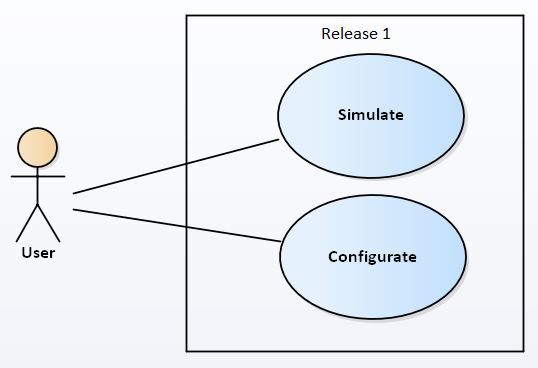
\includegraphics[width=0.9\textwidth]{img/UseCase_Diagram.JPG}
	\caption{Use Case Diagram}
	\label{img:UseCase_Diagram}
\end{figure}

\chapter{Logical View:}

\begin{figure}[H]
	\centering
	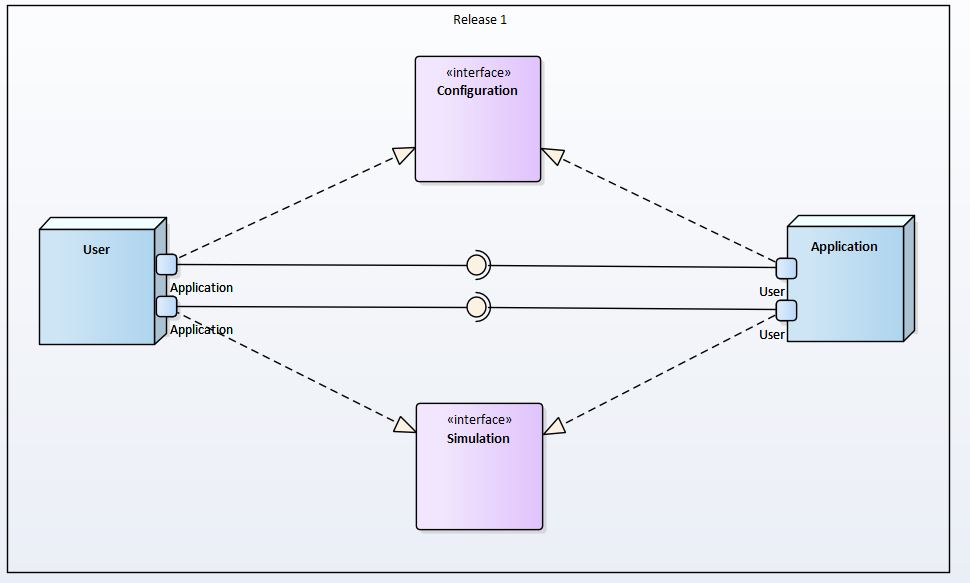
\includegraphics[width=0.9\textwidth]{img/LogicalView.JPG}
	\caption{Use Case Diagram}
	\label{img:LogicalView}
\end{figure}

\chapter{Application Deployment Diagram:}

\begin{figure}[H]
	\centering
	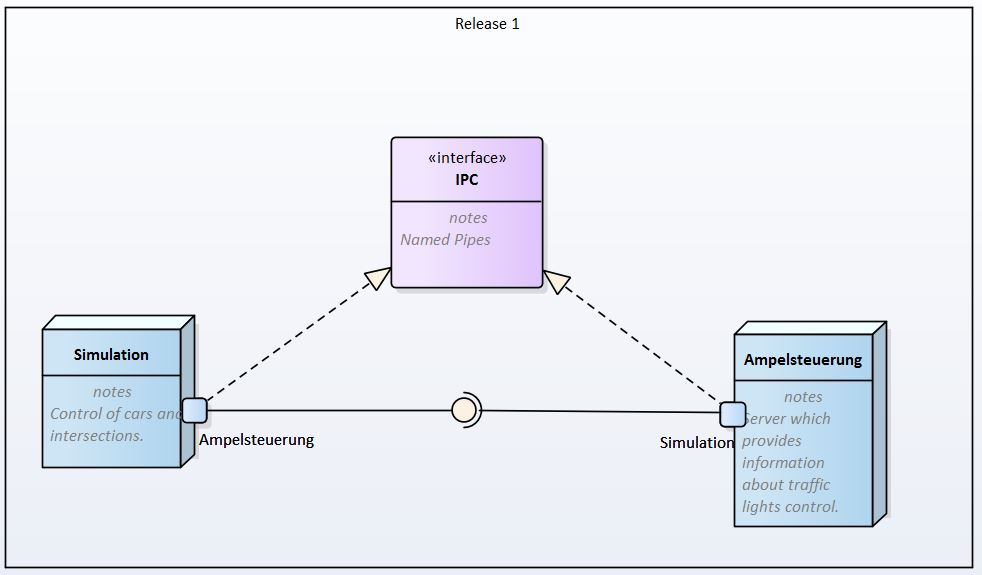
\includegraphics[width=0.9\textwidth]{img/Application_Deployment_Diagram.JPG}
	\caption{Use Case Diagram}
	\label{img:Application_Deployment_Diagram}
\end{figure}

\chapter{Simulation Component Diagram:}

\begin{figure}[H]
	\centering
	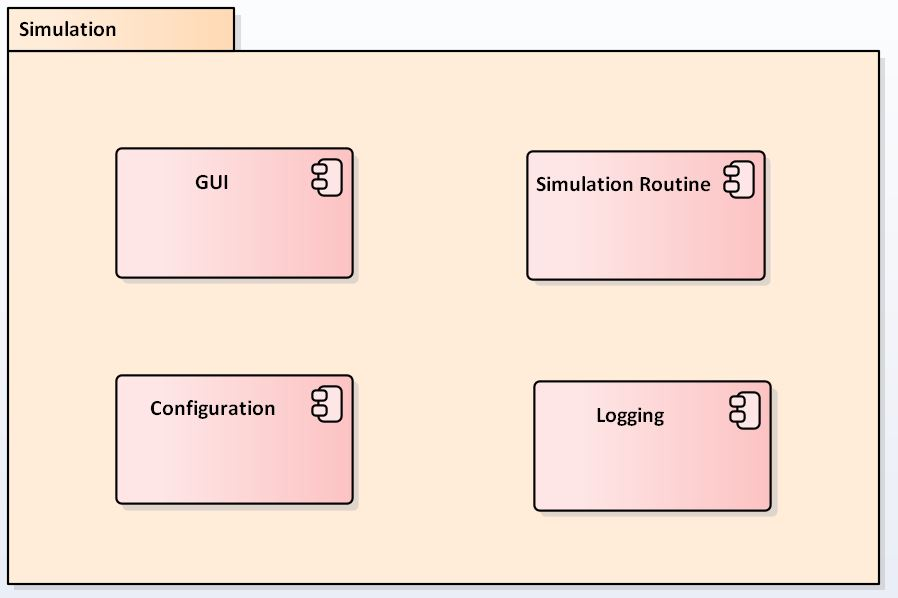
\includegraphics[width=0.9\textwidth]{img/Simulation_Component_Diagram.JPG}
	\caption{Use Case Diagram}
	\label{img:Simulation_Component_Diagram}
\end{figure}

\chapter{Traffic Lights Component Diagram:}

\begin{figure}[H]
	\centering
	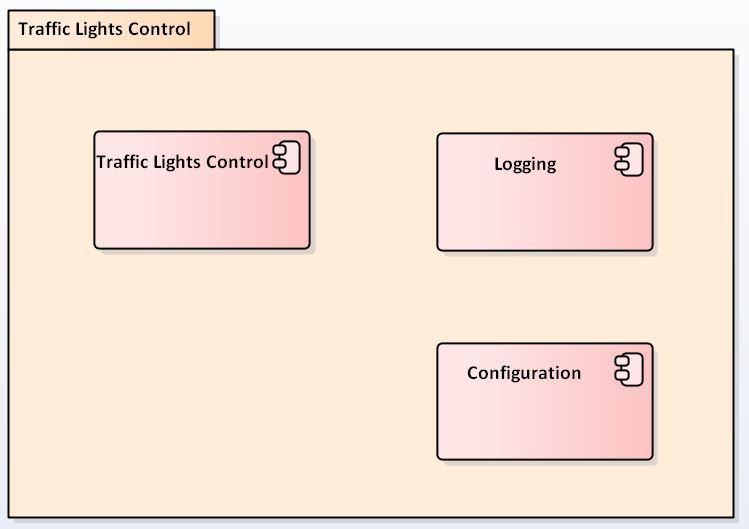
\includegraphics[width=0.9\textwidth]{img/TrafficLights_Component_Diagram.JPG}
	\caption{Use Case Diagram}
	\label{img:TrafficLights_Component_Diagram}
\end{figure}

\textbf{\textless{}Diagramm oder Tabelle\textgreater{}}

\textbf{\textless{}optional: Erläuterung der externen technischen
Schnittstellen\textgreater{}}

\textbf{\textless{}Mapping fachliche auf technische
Schnittstellen\textgreater{}}

\subsection{Lösungsstrategie}\label{section-solution-strategy}

\subsection{Bausteinsicht}\label{section-building-block-view}

\subsubsection{Whitebox Gesamtsystem}\label{_whitebox_gesamtsystem}

\emph{\textbf{\textless{}Übersichtsdiagramm\textgreater{}}}

\begin{description}
\item[Begründung]
\emph{\textless{}Erläuternder Text\textgreater{}}
\item[Enthaltene Bausteine]
\emph{\textless{}Beschreibung der enhaltenen Bausteine
(Blackboxen)\textgreater{}}
\item[Wichtige Schnittstellen]
\emph{\textless{}Beschreibung wichtiger Schnittstellen\textgreater{}}
\end{description}

%\subsubsubsection{\textless{}Name Blackbox 1\textgreater{}}\label{__name_blackbox_1}

%\emph{\textless{}Zweck/Verantwortung\textgreater{}}

%\emph{\textless{}Schnittstelle(n)\textgreater{}}

%\emph{\textless{}(Optional) Qualitäts-/Leistungsmerkmale\textgreater{}}

%\emph{\textless{}(Optional) Ablageort/Datei(en)\textgreater{}}

%\emph{\textless{}(Optional) Erfüllte Anforderungen\textgreater{}}

%\emph{\textless{}(optional) Offene Punkte/Probleme/Risiken\textgreater{}}

%\subsubsubsection{\textless{}Name Blackbox 2\textgreater{}}\label{__name_blackbox_2}

%\emph{\textless{}Blackbox-Template\textgreater{}}

%\subsubsubsection{\textless{}Name Blackbox n\textgreater{}}\label{__name_blackbox_n}

%\emph{\textless{}Blackbox-Template\textgreater{}}

%\subsubsubsection{\textless{}Name Schnittstelle 1\textgreater{}}\label{__name_schnittstelle_1}

%\ldots{}

%\subsubsubsection{\textless{}Name Schnittstelle \textgreater{}}\label{__name_schnittstelle_m}

%\subsubsection{Ebene 2}\label{_ebene_2}

%\subsubsubsection{\texorpdfstring{Whitebox \emph{\textless{}Baustein 1\textgreater{}}}{Whitebox \textless{}Baustein 1\textgreater{}}}\label{_whitebox_emphasis_baustein_1_emphasis}

%\emph{\textless{}Whitebox-Template\textgreater{}}

%\subsubsubsection{\texorpdfstring{Whitebox \emph{\textless{}Baustein 2\textgreater{}}}{Whitebox \textless{}Baustein 2\textgreater{}}}\label{_whitebox_emphasis_baustein_2_emphasis}

%\emph{\textless{}Whitebox-Template\textgreater{}}

%\ldots{}

%\subsubsubsection{\texorpdfstring{Whitebox \emph{\textless{}Baustein m\textgreater{}}}{Whitebox \textless{}Baustein m\textgreater{}}}\label{_whitebox_emphasis_baustein_m_emphasis}

%\emph{\textless{}Whitebox-Template\textgreater{}}

%\subsubsection{Ebene 3}\label{_ebene_3}

%\subsubsubsection{Whitebox \textless{}\_Baustein x.1\_\textgreater{}}\label{_whitebox_baustein_x_1}

%\emph{\textless{}Whitebox-Template\textgreater{}}

%\subsubsubsection{Whitebox \textless{}\_Baustein x.2\_\textgreater{}}\label{_whitebox_baustein_x_2}

%\emph{\textless{}Whitebox-Template\textgreater{}}

%\subsubsubsection{Whitebox \textless{}\_Baustein y.1\_\textgreater{}}\label{_whitebox_baustein_y_1}

%\emph{\textless{}Whitebox-Template\textgreater{}}

\subsection{Laufzeitsicht}\label{section-runtime-view}

\subsubsection{\texorpdfstring{\emph{\textless{}Bezeichnung
Laufzeitszenario
1\textgreater{}}}{\textless{}Bezeichnung Laufzeitszenario 1\textgreater{}}}\label{__emphasis_bezeichnung_laufzeitszenario_1_emphasis}

\begin{itemize}
\item
  \textless{}hier Laufzeitdiagramm oder Ablaufbeschreibung
  einfügen\textgreater{}
\item
  \textless{}hier Besonderheiten bei dem Zusammenspiel der Bausteine in
  diesem Szenario erläutern\textgreater{}
\end{itemize}

\subsubsection{\texorpdfstring{\emph{\textless{}Bezeichnung
Laufzeitszenario
2\textgreater{}}}{\textless{}Bezeichnung Laufzeitszenario 2\textgreater{}}}\label{__emphasis_bezeichnung_laufzeitszenario_2_emphasis}

\ldots{}

\subsubsection{\texorpdfstring{\emph{\textless{}Bezeichnung
Laufzeitszenario
n\textgreater{}}}{\textless{}Bezeichnung Laufzeitszenario n\textgreater{}}}\label{__emphasis_bezeichnung_laufzeitszenario_n_emphasis}

\ldots{}

\subsection{Verteilungssicht}\label{section-deployment-view}

\subsubsection{Infrastruktur Ebene 1}\label{_infrastruktur_ebene_1}

\emph{\textbf{\textless{}Übersichtsdiagramm\textgreater{}}}

\begin{description}
\item[Begründung]
\emph{\textless{}Erläuternder Text\textgreater{}}
\item[Qualitäts- und/oder Leistungsmerkmale]
\emph{\textless{}Erläuternder Text\textgreater{}}
\item[Zuordnung von Bausteinen zu Infrastruktur]
\emph{\textless{}Beschreibung der Zuordnung\textgreater{}}
\end{description}

\subsubsection{Infrastruktur Ebene 2}\label{_infrastruktur_ebene_2}

%\subsubsubsection{\texorpdfstring{\emph{\textless{}Infrastrukturelement 1\textgreater{}}}{\textless{}Infrastrukturelement 1\textgreater{}}}\label{__emphasis_infrastrukturelement_1_emphasis}

%\emph{\textless{}Diagramm + Erläuterungen\textgreater{}}

%\subsubsubsection{\texorpdfstring{\emph{\textless{}Infrastrukturelement 2\textgreater{}}}{\textless{}Infrastrukturelement 2\textgreater{}}}\label{__emphasis_infrastrukturelement_2_emphasis}

%\emph{\textless{}Diagramm + Erläuterungen\textgreater{}}

%\ldots{}

%\subsubsubsection{\texorpdfstring{\emph{\textless{}Infrastrukturelement n\textgreater{}}}{\textless{}Infrastrukturelement n\textgreater{}}}\label{__emphasis_infrastrukturelement_n_emphasis}

%\emph{\textless{}Diagramm + Erläuterungen\textgreater{}}

\subsection{Querschnittliche Konzepte}\label{section-concepts}

\subsubsection{\texorpdfstring{\emph{\textless{}Konzept
1\textgreater{}}}{\textless{}Konzept 1\textgreater{}}}\label{__emphasis_konzept_1_emphasis}

\emph{\textless{}Erklärung\textgreater{}}

\subsubsection{\texorpdfstring{\emph{\textless{}Konzept
2\textgreater{}}}{\textless{}Konzept 2\textgreater{}}}\label{__emphasis_konzept_2_emphasis}

\emph{\textless{}Erklärung\textgreater{}}

\ldots{}

\subsubsection{\texorpdfstring{\emph{\textless{}Konzept
n\textgreater{}}}{\textless{}Konzept n\textgreater{}}}\label{__emphasis_konzept_n_emphasis}

\emph{\textless{}Erklärung\textgreater{}}

\subsection{Entwurfsentscheidungen}\label{section-design-decisions}

\subsection{Qualitätsanforderungen}\label{section-quality-scenarios}

\subsubsection{Qualitätsbaum}\label{_qualit_tsbaum}

\subsubsection{Qualitätsszenarien}\label{_qualit_tsszenarien}

\subsection{Risiken und technische Schulden}\label{section-technical-risks}

\subsection{Glossar}\label{section-glossary}

\begin{longtable}[]{@{}ll@{}}
\toprule
\begin{minipage}[b]{0.31\columnwidth}\raggedright\strut
Begriff\strut
\end{minipage} & \begin{minipage}[b]{0.63\columnwidth}\raggedright\strut
Definition\strut
\end{minipage}\tabularnewline
\midrule
\endhead
\begin{minipage}[t]{0.31\columnwidth}\raggedright\strut
\emph{\textless{}Begriff-1\textgreater{}}\strut
\end{minipage} & \begin{minipage}[t]{0.63\columnwidth}\raggedright\strut
\emph{\textless{}Definition-1\textgreater{}}\strut
\end{minipage}\tabularnewline
\begin{minipage}[t]{0.31\columnwidth}\raggedright\strut
\emph{\textless{}Begriff-2}\strut
\end{minipage} & \begin{minipage}[t]{0.63\columnwidth}\raggedright\strut
\emph{\textless{}Definition-2\textgreater{}}\strut
\end{minipage}\tabularnewline
\bottomrule
\end{longtable}




%--- Begin generated contents ---
%\input{latex/Bankmanagement_8h.tex}
%--- End generated contents ---

% Index

\newpage
\phantomsection
\clearemptydoublepage
\addcontentsline{toc}{chapter}{Index}
\printindex

\end{document}
